\documentclass{article}

\PassOptionsToPackage{square, numbers}{natbib}

% ready for submission
% \usepackage{neurips_2023}

% to compile a preprint version, e.g., for submission to arXiv, add add the
% [preprint] option:
\usepackage[preprint]{neurips_2023}

% to compile a camera-ready version, add the [final] option, e.g.:
% \usepackage[final]{neurips_2023}

\usepackage[utf8]{inputenc}             % allow utf-8 input
\usepackage[T1]{fontenc}                % use 8-bit T1 fonts
\usepackage[colorlinks=true]{hyperref}  % hyperlinks
\usepackage{url}                        % simple URL typesetting
\usepackage{booktabs}                   % professional-quality tables
\usepackage{amsfonts}                   % blackboard math symbols
\usepackage{nicefrac}                   % compact symbols for 1/2, etc.
\usepackage{microtype}                  % microtypog raphy
\usepackage{xcolor}                     % colors
\usepackage{graphicx}                   % figures

\bibliographystyle{abbrvnat}
\graphicspath{{figures}}

\title{QwinSR: An MLP-based Shifted Window Model for Image Super Resolution}

\author{
  Mark Bauer \\
  Grainger College of Engineering\\
  University of Illinois Urbana-Champaign\\
  \texttt{markb5@illinois.edu} \\
  \And
  Quinn Ouyang\thanks{"QwinSR" is a play on Swin using Quinn's name. This was Mark's idea.} \\
  College of Fine and Applied Arts \\
  University of Illinois Urbana-Champaign \\
  \texttt{qouyang3@illinois.edu} \\
}

\begin{document}

\maketitle

\begin{abstract}
    Famous for its shifted window representation, the Swin Transformer backbone architecture has consistently showcased state-of-the-art performance across a range of well-established computer vision benchmarks. To enhance computational efficiency, the Swin Mixer architecture adopts this structure but substitutes its attention layers with simpler multi-layer perceptrons (MLPs). In line with this design, we introduce QwinSR, an application of this all-MLP architecture tailored for single image super-resolution. This adaptation simplifies the Swin Transformer-based image restoration model, SwinIR. QwinSR leverages MLPs to extract essential features and subsequently aggregates them within a compact convolutional neural network, facilitating image reconstruction. We anticipate that our model will yield competitive accuracy-to-computation metrics, particularly when compared to SwinIR and other leading models in the field. Our (untested) code is available at \url{https://github.com/quinnouyang/QwinSR}.
\end{abstract}

\section{Introduction}

Despite advances in modern photography and image transmission technology, resolution loss is often an unavoidable or necessary compromise. This produces a need and desire for techniques to construct higher fidelity images from lower resolution sources, which we call super resolution (SR) imaging \citep{Overview, ESRGAN}. However, SR is a more niche category than other computer vision tasks (such as classification and semantic segmentation) \citep{PapersWithCode}, making this field ripe for new research. Given the simple objective and need for research on SR, we propose a simplified MLP-based model on the shifted window design from the Swin Transformer by \citet{SwinTransformer}: QwinSR.

\subsection{Related Work}

\subsubsection{Single Image Super-Resolution}

“Super-resolution” generally refers to the process of enhancing the visual detail and fidelity of an image by predicting pixels to increase its resolution. In other literature, SR is roughly interchangeable with the more general terms “upsampling” and “reconstruction” \citep{Overview, ESRGAN}. Note that the latter implies that an exact / true higher resolution image exists for a lower resolution one, which typically comes from artificial downsampling; this setup is known as "classic image SR" \citep{SRGAN, SwinIR}. Unlike the more common variant of this task, multiple image SR, “single image” specifically refers to a process that relies on only one source image rather than several. Effective multiple image SR techniques exploit the related images for more pixel information to construct from, which can apply in the real-world (e.g. a burst shot, video frames, etc.) \citep{Overview, DLSS}. However, we focus on single image SR as it is a more fundamental and challenging task \citep{DLSS}.

Traditional algorithmic approaches for SR directly interpolate pixels from a lower resolution source, typically assuming a downsampling process to generalize the reconstruction. Popular basic algorithms include bicubic and nearest-neighbor interpolation which are fast and eschew the long training times associated with learning-based models, but the absence of trained priors obviously limits their ability to hallucinate new pixels \citep{Overview, DLSS}.

\subsubsection{Learning-based Approaches}

On the other hand, learning-based models spanning a variety of architectures have far surpassed the generalized interpolations that traditional approaches limit themselves to. Models based on convolutional neural networks (e.g. SRCNN, SRResNet), general adversarial networks (e.g. ESRGAN, SRGAN, Real-ESRGAN), and transformers (e.g. SwinIR) have all competed effectively for state-of-the-art performance \citep{SRCNN, SRGAN, ESRGAN, SwinIR}.

\begin{figure}\label{fig:example}
    \centering
    \begin{tabular}{c c c c}
        
\includegraphics[width=80pt]{bicubic.png} & 
\includegraphics[width=80pt]{srresnet.png} & 
\includegraphics[width=80pt]{srgan.png} & 
\includegraphics[width=80pt]{original.png} \\
        \small Bicubic Interpolation              & \small SRResNet                            & \small SRGAN                            & \small Original
    \end{tabular}
    \caption{Visual comparisons of traditional and learning-based classic image SR approaches to a $\times 4$-upscaled original high resolution image.}
\end{figure}

For SR related tasks, CNNs are effective at global feature extraction but have lately been usurped by transformers, which tend to be more robust and lightweight. As a consequence, pure CNN models often require added complexity just to match the performance of transformer models \citep{MLPMixer}. This is especially a concern as CNNs typically scale quadratically to input images. Hence, utilizing hybrid CNN-transformer models can be quite effective in improving costs, where CNNs perform global feature extraction while transformers focus on local feature extraction. SwinIR demonstrates this through its low and high frequency extractions \citep{SwinIR}.

GANs tend to be tedious to fine tune and also have many trainable parameters, making the training process very long \citep{SRGAN}. Similarly, diffusion-based models such as StableSR from \citet{StableSR} have gigantic datasets and are quite complex. The focus of this research project is on simplicity rather than extreme predictive performance, and as such we do not consider these models.

\subsubsection{All-MLP}

“All-MLP” describes a model as primarily relying on only multi-layer perceptrons (MLPs), often in contrast to neural networks or transformers. These models tend to have significantly fewer parameters and simpler architectures than other models, offering an ideal tradeoff between accuracy and training time / running time \citep{SwinTransformer,MLPMixer}. Proposed by \citet{MLPMixer}, the MLP-Mixer is one of the first all-MLP demonstrations for computer vision. Despite its apparent computational limitations, MLP-Mixer has boasted results comparable to those from state-of-the-art implementations for image classification \citep{MLPMixer}. Inspired by this work, we chose to follow the same all-MLP design philosophy and apply it to SR as a more high level benchmark. While QwinSR uses Mixer Layers for deep feature extraction, its shallow feature extraction and image reconstruction still relies on CNNs. Hence, we can characterize it as a hybrid CNN-MLP model rather than a true all-MLP one.

\subsubsection{Shifted Window}

\paragraph{Swin Transformer:} First popularized by \citet{SwinTransformer}, the shifted window approach is the computational representation in a groundbreaking computer vision model: the Swin Transformer. Critically, it limits “self-attention computation to non-overlapping local windows while also allowing for cross-window connection,” eliminating global self-attention and thus reducing from quadratic to linear computational complexity relative to image size \citep{SwinTransformer}. Variants of the Swin Transformer have achieved state-of-the-art results in a variety of common tasks, including image classification and semantic segmentation \citep{SwinIR, SwinSeg}.

\paragraph{Swin-Mixer:} The modularity of the shifted window technique in the Swin Transformer enables replacing its attention layers with MLPs, yielding the Swin-Mixer. Specifically, it replaces each of its multi-head attention layers with the all-MLP layers presented by Tolstikhin et al., converting the Swin Transformer Blocks into Swin Mixer Blocks. Swin-Mixer surpasses the already classification results of MLP-Mixer and other all-MLP models \citep{SwinTransformer,MLPMixer}, but little research exists on how it performs elsewhere, e.g. in SR.

\paragraph{SwinIR:} A pioneering model for attention-based SR, SwinIR uses basic convolutional layers for shallow feature extraction and Swin Transformer blocks for deep feature extraction. These extracted features are then passed through a basic upsampling convolution that involves a convolutional layer and a pixel shuffle. SwinIR impressively surpasses other top-performing models based on CNNs, GANs, etc. in classical SR \citep{SwinIR}.

\section{Model Architecture}

The architecture of QwinSR is novel in that it combines the model architectures of SwinIR and Swin-Mixer. Similar to other state-of-the-art SR models such as SRResNet, ESRGAN, and SwinIR, our model involves a 3 step architecture: shallow feature extraction, deep feature extraction, and image reconstruction \citep{SwinIR, ESRGAN}. (See Figure~\ref{fig:architecture}.)

\begin{figure}
    \centering
    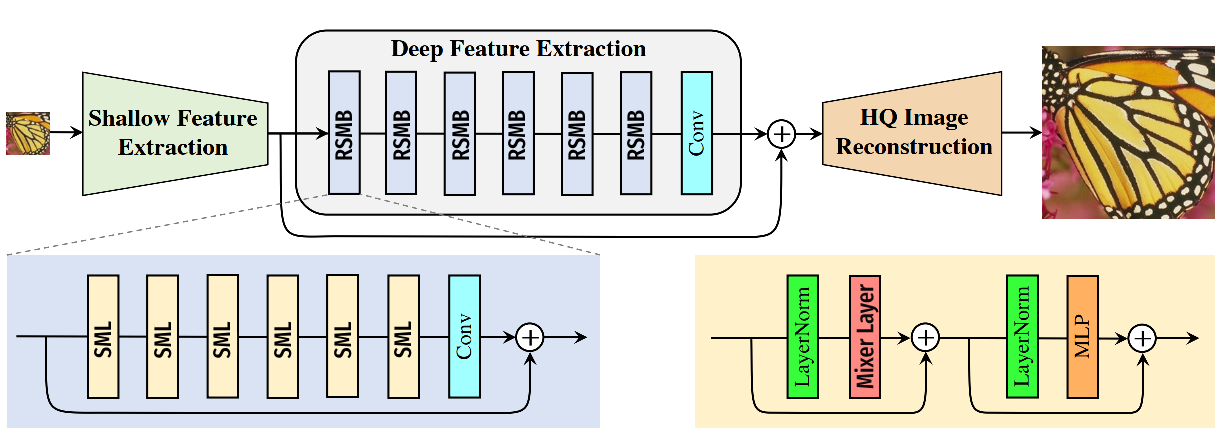
\includegraphics[width=\textwidth]{qwinir-architecture.png}
    \caption{The architecture of QwinSR. Figure based off of that of \citet{SwinIR}.}
    \label{fig:architecture}
\end{figure}

\subsection{Shallow Feature Extraction}

QwinSR uses the exact same method for shallow feature extraction as SwinIR. That is, given a low quality input image, we use a $3 \times 3$ convolutional layer to perform shallow feature extraction. Convolutional layers are effective for performing local feature extraction, making this step useful in preserving low-frequency information at the early stages of processing. Liang et al, also note that the use of this layer not only leads to more stable optimization and better results, but also provides a simple way of mapping input images to higher dimensional feature spaces \citep{SwinIR}.

\subsection{Deep Feature Extraction}

\begin{figure}
    \centering
    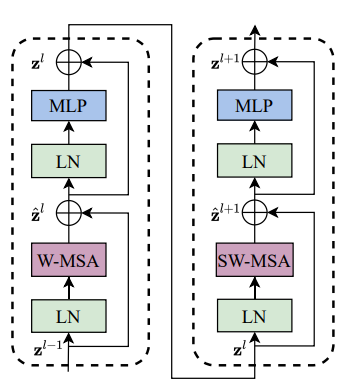
\includegraphics[width=100pt]{swin-transformer-block.png}
    \caption{Two original successive Swin Transformer blocks with attention heads included (W-MSA and SW-MSA). Swin Mixer blocks replace each of these with a Mixer Layer \citep{SwinTransformer}.}
    \label{fig:transformer}
\end{figure}

\paragraph{Swin Mixer Blocks and Layers:} We perform deep feature extraction by passing the extracted shallow features through a series of 6 Residual Swin Mixer Blocks (RSMBs) and a $3 \times 3$ convolutional layer. These blocks are residual because they each contain a skip connection, where the results of each block are aggregated with the input features passed to the block. Each RSMB contains a series of 6 Swin Mixer Layers (SMLs) followed by a $3 \times 3$ convolutional layer, and each SML is simply a Swin Transformer Layer that has had its multi-head self attention module replaced with a Mixer Layer, as we depict in Figure~\ref{fig:transformer} \citep{MLPMixer,SwinTransformer}.

\paragraph{Mixer Layer:} As \citet{MLPMixer} describes each mixer layer (See Figure~\ref{fig:mixer}.) is composed of 2 MLPs: one channel-mixing MLP and one token-mixing MLP. Each MLP consists of two fully connected layers between a GELU nonlinearity. The channel-mixing MLP operates first, which allows communication between different input channels (i.e. windows) and operates on each input token (i.e. pixels within windows) independently. The results of the channel-mixing MLPs are passed to the token-mixing MLPs, which allow communication between different tokens and operate on each channel independently \citep{MLPMixer}.

By utilizing this mixing architecture, we can extract features without explicitly requiring attention. Hence, it makes sense for deep feature extraction to be accurate even when attention heads in the Swin Transformer blocks are replaced with Mixer Layers \citep{MLPMixer}. However, due to the removal of attention heads, these blocks are technically no longer transformers, which is why we refer to them as Swin Mixer Blocks in our model.

\begin{figure}
    \centering
    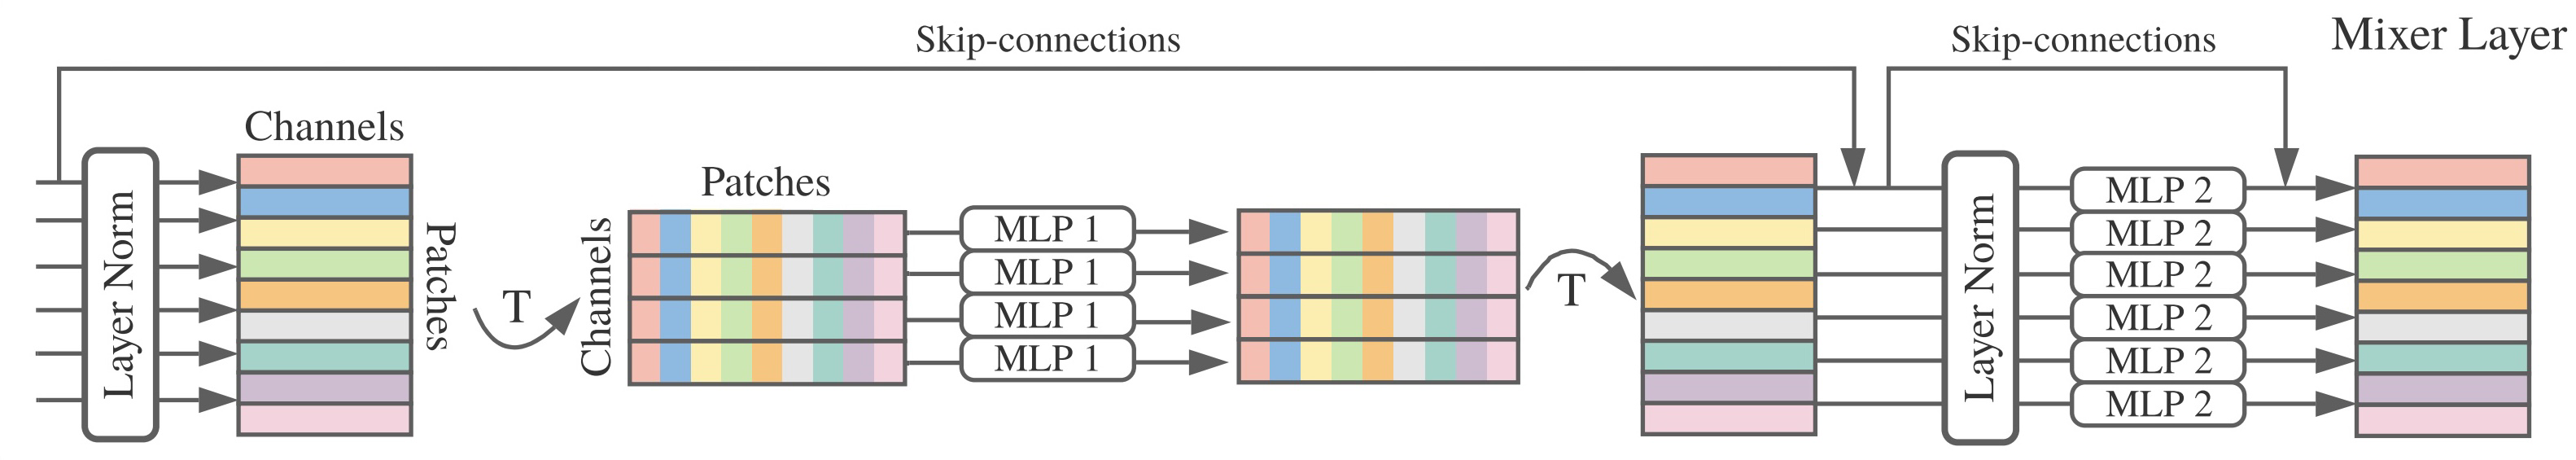
\includegraphics[width=\textwidth]{mixer-layer.png}
    \caption{Mixer layer from MLP-Mixer, consisting of token-mixing MLP, channel-mixing MLP, skip-connections, dropout, and layer normalization \citep{MLPMixer}.}
    \label{fig:mixer}
\end{figure}

\subsection{Reconstruction}

\paragraph{Skip Connection:} Using a skip connection, we aggregate the originally extracted shallow features and the newly extracted deep features and pass them into an image reconstruction module. The skip connection ensures that low frequency features are not lost during the reconstruction process \citep{SwinIR}.

\paragraph{Convolution Reconstruction Module:} We implement a sub-pixel convolutional neural network proposed by Shi et al. as ESPCN (See Figure~\ref{fig:escpn}.), the same technique utilized by SwinIR \citep{SwinIR, ESPCN}. ESPCN consists of two convolution layers for feature extraction and a sub-pixel convolution layer that aggregates the low resolution features. From here, it then constructs the high resolution image in a single step \citep{SwinIR, ESPCN}.


\begin{figure}
    \centering
    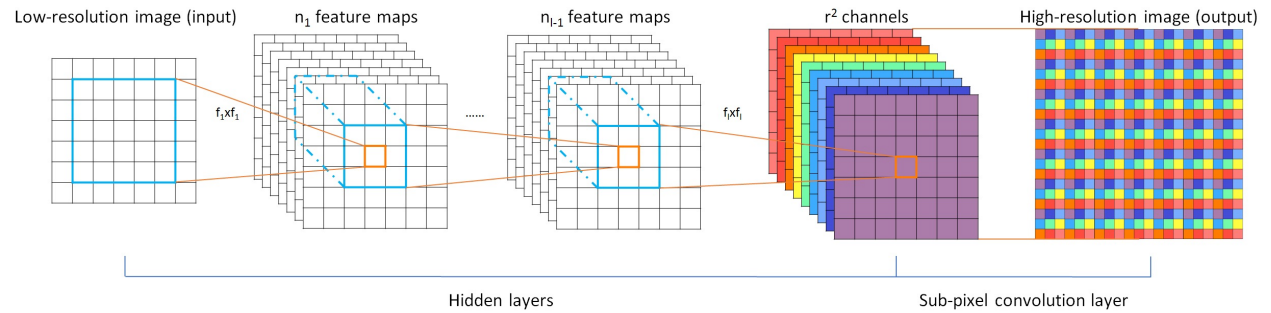
\includegraphics[width=\textwidth]{espcn.png}
    \caption{The network architecture for ESPCN \citep{ESPCN}.}
    \label{fig:escpn}
\end{figure}

\section{Experiments}

Unfortunately, we were unable to conduct a formal experimental procedure due to resource and time constraints. However, barring those factors, we would replicate the experiments performed by Liang et al. as our model derives from the SwinIR architecture. It is also worth noting that SwinIR's experimental procedure consists of image super resolution, image denoising, and JPEG compression artifact reduction. Since our architecture focuses only on super resolution, we ignore the latter two experimental components.

\subsection{Ablation Study}

The first stage of our experimental procedure will be an ablation study, which involves altering and removing certain components from our model to understand the contributions of those components to our results. We train our model on the DIV2K \citep{Div2K} dataset and test the Manga109 \citep{Manga109} dataset.

The first portion of this stage will observe the effects of changing the channel number, number of Swin Mixer Blocks, and number of SMLs per block on model performance. To perform this step, we will test a variety of combinations for values of these hyperparameters and observe the relative correlations between the values of each hyperparameter and peak signal to noise ratio (PSNR) for the upscaled images.

The second portion of this stage will observe the effects of changing patch size and the number of training images. To perform this step, we will test a variety of combinations for values of these hyperparameters and observe how each value affects PSNR and time for convergence.

The third portion of this stage will observe the effects of the residual connection and convolutional layer in each SMB. Like in the SwinIR paper, we will test 4 residual connection variants in each block: no residual connection (i.e. no convolution operation), a $1 \times 1$ convolution layer, a $3 \times 3$ convolution layer, and three $3 \times 3$ convolution layers. For each of these hyperparameter values, the corresponding PSNRs will be assessed and compared.

\subsection{Performance Benchmarks}

In the second stage of our experimental procedure, we will select the optimal combination of hyperparameters as determined in the previous stage, and we will use them to test our model on the Set5 \citep{Set5}, Set14 \citep{Set14}, BSD100 \citep{BSD100}, Urban100 \citep{Urban100}, and Manga109 \citep{Manga109} datasets. The benchmarks we record in this stage will be PSNR (peak signal to noise ratio, lower indicates less grainy output images), SSIM (structural similarity index measure, which compares how similar an upscaled image is to the original high quality image a model seeks to reproduce), the number of model parameters, and the number of multiply-accumulate operations.

These measurements will be compared to the benchmarks recorded in the SwinIR paper (this is convenient, because the SwinIR paper contains benchmarks for numerous SOTA architectures, not just for the SwinIR architecture). By performing this comparison, we will gain conclusive evidence as to how our model performs relative to state of the art models–in particular, if our model has a viable accuracy/cost ratio.

\section{Conclusion}

In this paper, we propose QwinSR, an image restoration model that combines the architectures of SwinIR and Swin-Mixer. Like SwinIR, this model consists of three phases: shallow feature extraction, deep feature extraction, and image reconstruction. Unlike SwinIR, our model uses residual Swin Mixer Blocks for deep feature extraction, where each block consists of Swin-Mixer layers, a convolution layer, and a residual connection. While we were unable to conduct a formal experimental phase due to resource and time constraints, we believe that this model has the potential to perform at a similar level to state of the art image upscaling models.

For future work, we would like to conduct a formal testing phase on a more substantial cluster of GPUS, as GCP and our personal computers proved to be insufficient for training our model. Furthermore, we would like to experiment with the placement of skip connections within our network to potentially remove the need for an initial convolutional layer for shallow feature extraction, similar to the SwinSeg architecture described by \citet{SwinSeg}.


\begin{ack}
    We would like to acknowledge Paris Smaragdis, Krishan Subramani (please be gentle to us), Evan Matthews, Nicolas Prate, and Quinn’s sister’s cat, Sesame.

    We have no funding.
\end{ack}

\bibliography{baby}

\end{document}